\documentclass[a4, 12pt]{article}
\usepackage[a4paper,top=1.3cm,bottom=2cm,left=1.5cm,right=1.5cm,marginparwidth=0.75cm]{geometry}
\usepackage{setspace}
\usepackage{cmap}
\usepackage{mathtext}
\usepackage[utf8]{inputenc}
\usepackage[english,russian]{babel}
\usepackage[T2A]{fontenc}
\usepackage{multirow}
\usepackage{graphicx}
\usepackage{wrapfig}
\usepackage{tabularx}
\usepackage{float}
\usepackage{longtable}
\usepackage{hyperref}
\hypersetup{colorlinks=true,urlcolor=blue}
\usepackage[rgb]{xcolor}
\usepackage{amsmath,amsfonts,amssymb,amsthm,mathtools}
\usepackage{icomma}
\mathtoolsset{showonlyrefs=true}
\usepackage{euscript}
\usepackage{mathrsfs}

\DeclareMathOperator{\sgn}{\mathop{sgn}}
\newcommand*{\hm}[1]{#1\nobreak\discretionary{}
	{\hbox{$\mathsurround=0pt #1$}}{}}


\title{\textbf{Измерение модуля Юнга стержней методом акустического резонанса. (1.4.8)}}
\author{Балдин Виктор Б01-303}
\date{20 ноября 2023}


\begin{document}

	\maketitle

	\section{Введение}
    \textbf{Цель работы:} исследовать явление акустического резонанса в тонком стержне; из-
мерить скорость распространения продольных звуковых колебаний в тонких стержнях из различных материалов и различных размеров; измерить модули Юнга раз-
личных материалов.\\
\textbf{В работе используются:} генератор звуковых частот, частотомер, осциллограф,
электромагнитные излучатель и приёмник колебаний, набор стержней из различных материалов.

    \section{Теоретическая часть}
    Основной характеристикой упругих свойств твёрдого тела является его
модуль Юнга $E$. Согласно закону Гука, если к элементу среды приложено
некоторое механическое напряжение $\sigma$, действующее вдоль некоторой
оси $x$ (напряжения по другим осям при этом отсутствуют), то в этом эле-
менте возникнет относительная деформацию вдоль этой же оси
$\varepsilon = \Delta x/x_0$ , определяемая соотношением
\begin{equation}
    \sigma = \varepsilon E
\end{equation}
Если с помощью кратковременного воздействия в некотором элементе
твёрдого тела создать малую деформацию, она будет далее распростра-
няться в среде в форме волны, которую называют акустической или звуко-
вой. Распространение акустических волн обеспечивается за счёт упругости
и инерции среды. Волны сжатия/растяжения, распространяющиеся вдоль
оси, по которой происходит деформация, называются продольными. Как
будет строго показано далее, скорость $u$ распространения продольной аку-
стической волны в простейшем случае длинного тонкого стержня опреде-
ляется соотношением
\begin{equation}
    u = \sqrt{\frac{E}{\rho}}
\end{equation}
где $\rho$ — плотность среды.
Заметим, что размерность модуля Юнга $E$ равна [Н/м$^2$] и совпадает с
размерностью механического напряжения (или давления). Характерные
значения модуля Юнга металлов лежат в диапазоне $E\sim$ 1010 ÷ 1012 Па, так
что при плотности $\rho\sim$ 104 кг/м3 характерные значения скорости звука в
твёрдых телах составляют $u\sim$ 103 - 104 м/с.
В общем случае звуковые волны в твёрдых телах могут быть не только
продольными, но и поперечными — при этом возникает деформация сдвига
перпендикулярно распространению волны. Кроме того, описание распространения волн в неограниченных средах осложняется тем
обстоятельством, что при отличном от нуля коэффициенте Пуассона 1
напряжение вдоль одной из осей вызывает деформацию не только в про-
дольном, но и в поперечном направлении к этой оси. Таким образом, общее
описание звуковых волн в твёрдых телах — относительно непростая задача.
В данной работе мы ограничимся исследованием наиболее простого случая
упругих волн, распространяющихся в длинных тонких стержнях.
Рассмотрим стержень постоянного круглого сечения, радиус $R$ которого
много меньше его длины $L$. С точки зрения распространения волн стержень
можно считать тонким, если длина $\lambda$ звуковых волн в нём велика по срав-
нению с его радиусом: $\lambda R$. Такая волна может свободно распростра-
няться только вдоль стержня, поэтому можно считать, что стержень испы-
тывает деформации растяжения и сжатия только вдоль своей оси (заметим,
что в обратном пределе коротких волн $\lambda R$ стержень следует рассматри-
вать как безграничную сплошную среду). Если боковые стенки тонкого
стержня свободны (т.е. стержень не сжат с боков), то его деформации опи-
сывается законом Гука в форме (1), и, следовательно, его упругие свойства
определяются исключительно модулем Юнга среды.
Акустическая волна, распространяющаяся в стержне конечной длины $L$,
испытает отражение от торцов стержня. Если при этом на длине стержня
укладывается целое число полуволн, то отражённые волны будут склады-
ваться в фазе с падающими, что приведёт к резкому усилению амплитуды
их колебаний и возникновению акустического резонанса в стержне. Изме-
ряя соответствующие резонансные частоты, можно определить скорость
звуковой волны в стержне и, таким образом, измерить модуль Юнга мате-
риала стержня. Акустический метод является одним из наиболее точных
методов определения упругих характеристик твёрдых тел.
Получим дифференциальное уравнение, описывающее распростране-
ние упругих волн в тонком стержне.
Направим ось $x$ вдоль геометрической оси стержня (рис. 1). Разобьём
исходно недеформированный стержень на тонкие слои толщиной $\Delta x$. При
продольной деформации среды границы слоёв сместятся в некоторые но-
вые положения. Пусть плоскость среды, находящаяся исходно в точке $x$
\begin{figure}[H]
    \centering
    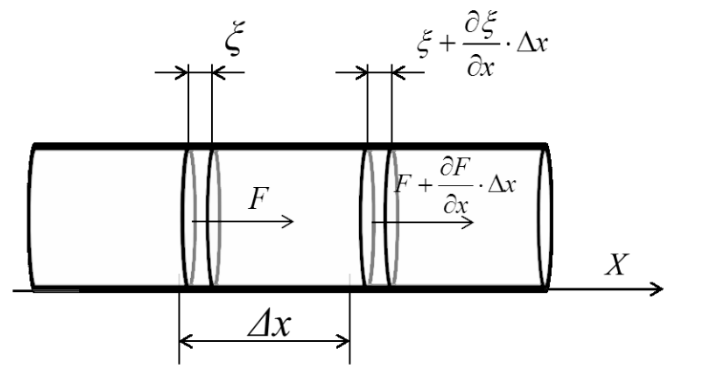
\includegraphics[scale = 1.5]{scheme.png}
    \caption{}
\end{figure}
сместилась к моменту $t$ на расстояние $\xi(x, t)$. Тогда слой, занимавший исходно
отрезок $[x, x+\Delta x]$, изменил свой продольный размер на величину $$\Delta \xi =
\frac{\partial \xi}{\partial x}\Delta x$$

\section{Методика измерений}
\begin{figure}[H]
    \centering
    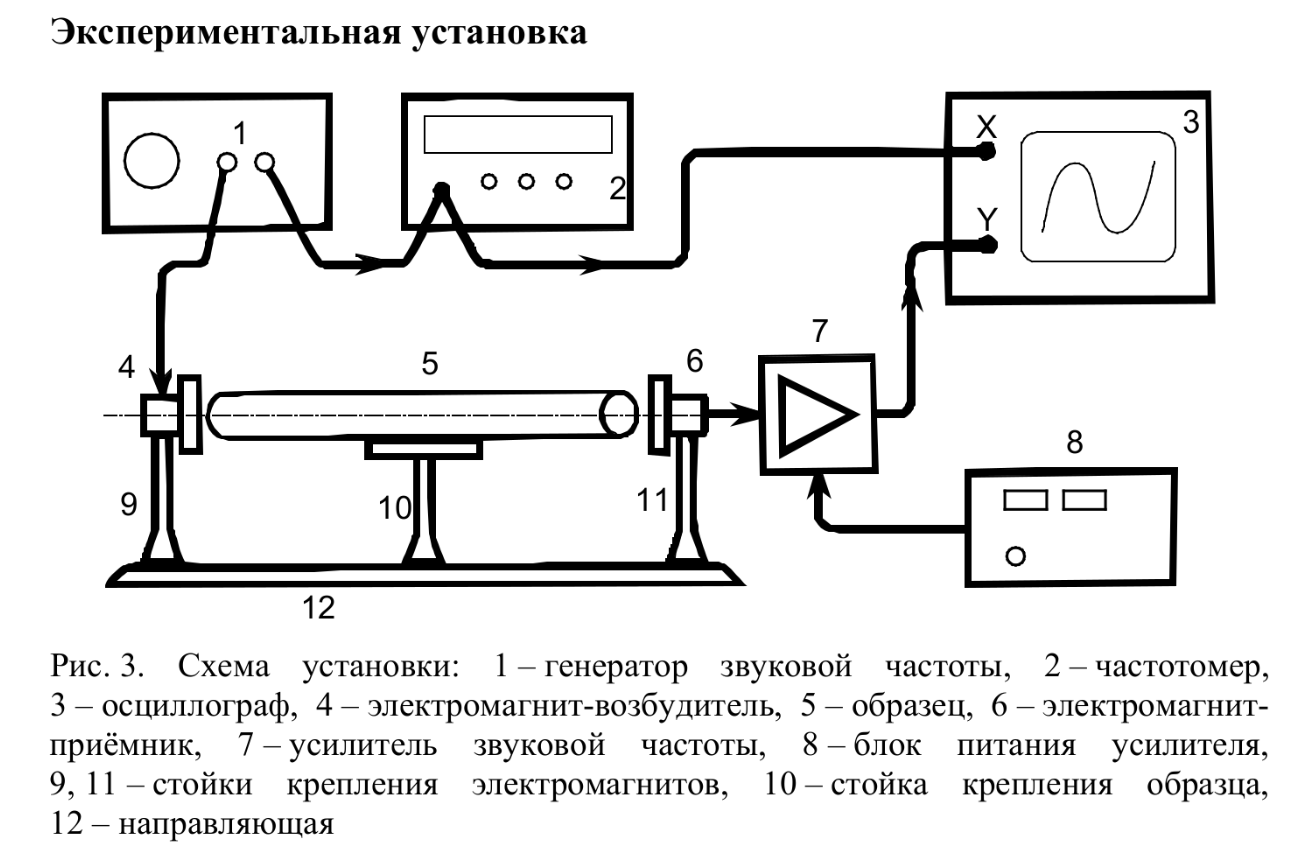
\includegraphics[scale = 1.5]{stand.png}
\end{figure}
Схема экспериментальной установки приведена на рис. 3. Исследуемый
стержень 5 размещается на стойке 10. Возбуждение и приём колебаний в
стержне осуществляются электромагнитными преобразователями 4 и 6,
расположенными рядом с торцами стержня. Крепления 9, 11 электро-
магнитов дают возможность регулировать их расположение по высоте, а
также перемещать вправо-влево по столу 12.
\par Электромагнит 4 служит для возбуждения упругих механических про-
дольных колебаний в стержне. На него с генератора звуковой частоты 1 по-
даётся сигнал синусоидальной формы: протекающий в катушке электро-
магнита ток создаёт пропорциональное ему магнитное поле, вызывающее
периодическое воздействие заданной частоты на торец стержня (к торцам
стержней из немагнитных материалов прикреплены тонкие стальные
шайбы). Рядом с другим торцом стержня находится аналогичный электро-
магнитный датчик 6, который служит для преобразования механических
колебаний в электрические. Принцип работы электромагнитных датчиков
описан подробнее ниже.
Сигнал с выхода генератора поступает на частотомер 2 и на вход
канала X осциллографа 3. ЭДС, возбуждаемая в регистрирующем электро-
магните 6, пропорциональная амплитуде колебаний торца стержня, усили-
вается усилителем 7 и подаётся на вход канала Y осциллографа.
Изменяя частоту генератора и наблюдая за амплитудой сигнала с реги-
стрирующего датчика, можно определить частоту акустического резонанса
в стержне. Наблюдения в режиме X–Y позволяют сравнить сигналы гене-
ратора и датчика, а также облегчает поиск резонанса при слабом сигнале.
\par Как следует из формулы (2), модуль Юнга материала $E$ может быть
найден по скорости распространения акустических волн в стержне $u$ и его
плотности $\rho$. Для определения скорости $u$ в данной работе используется
метод акустического резонанса. Это явление состоит в том, что при часто-
тах гармонического возбуждения, совпадающих с собственными частотами
колебаний стержня $f \approx f_\text{рез}/Q$ , резко увеличивается амплитуда колебаний, при
этом в стержне образуется стоячая волна.
Возбуждение продольных колебаний в стержне происходит посред-
ством воздействия на торец стержня периодической силой, направленной
вдоль его оси. Зная номер гармоники $n$ и соответствующую резонансную
частоту $f_n$ , на которой наблюдается усиление амплитуды колебаний,
можно вычислить скорость распространения продольных волн в стержне:
\begin{equation}
    u = 2L\frac{f_n}{n}
\end{equation}

Таким образом, для измерения скорости $u$ необходимо измерить длину
стержня $L$ и получить зависимость резонансной частоты от номера резо-
нанса $n$. Если все теоретические предположения справедливы, эта за-
висимость будет прямой пропорциональностью.
Следует отметить, что в реальном металлическом стержне могут воз-
буждаться не только продольные, но и поперечные (в частности, изгибные)
колебания стержня. При этом каждому типу колебаний соответствует не
одна, а целый спектр частот. Таким образом, стержень «резонирует» не
только на частотах, определяемых формулой (15), но и на множестве дру-
гих частот. Для того чтобы отличить нужные нам резонансные частоты от
«паразитных», следует провести предварительные расчёты и не принимать
во внимание резонансы, не описываемые зависимостью (15).
Скажем также несколько слов о точности измерения резонансной ча-
стоты. В первую очередь отметим, что в идеальном случае резонанс дости-
гался бы при строгом совпадении частот $f = f_n$ (а амплитуда в резонансе
стремилась бы к бесконечности). Однако в реальности возбуждение стоя-
чей волны возможно при относительно малом отклонении частоты от резо-
нансной — амплитуда колебаний как функция частоты $A(f)$ имеет резкий
максимум при $f = f_n$.
\par Именно конечная ширина резонанса $\Delta f$ определяет в основном погреш-
ность измерения частоты в нашем опыте.
Используемые в работе металлические стержни являются весьма высо-
кодобротными системами: их добротность оказывается порядка $Q\sim$ 102 ÷
÷ 103 . Поэтому ширина резонанса оказывается довольно малой, что приво-
дит к необходимости тонкой настройки частоты генератора (при $f\sim$
 5 кГц ширина резонанса $\Delta f$ оказывается порядка нескольких герц)
Кроме того, время установления резонансных колебаний, которое можно
оценить как
\begin{equation}
    \tau_\text{уст} \sim \frac{1}{\Delta f} \sim \frac{Q}{f},
\end{equation}
оказывается весьма велико, из-за чего поиск резонанса нужно проводить, меняя частоту
генератора очень медленно.
\section{Оборудование}
Генератор звуковых частот, частотомер, осциллограф,
электромагнитные излучатель и приёмник колебаний, набор стержней из различных материалов.

\section{Измерения и обработка результатов}
\begin{enumerate}
    \item Измерим плотность всех предоставленных нам материалов:
    \begin{table}[H]
        \centering
        \caption{Плотности}
        \begin{tabular}{c|c|c|c|}
            \hline
                            & Медь          & Дюралюминий      & Сталь \\
            \hline
             $\rho$, г/см$^3$ & $8.68\pm0.08$ & $2.71\pm0.03$ & $7.73\pm0.05$ \\
            \hline
        \end{tabular}
    \end{table}
    \item Включим генератор.
    \item Длина всех исследуемых стержней дана: $L = (600\pm0.5)\;\text{мм}$.
    \item Исследуем по порядку медный, дюралюминиевый и стальной стержни на
    резонанс.
    \begin{table}[H]
        \centering
        \caption{Найденные частоты резонансов в зависимости от номера резонанса}
        \begin{tabular}{|c|c|c|c|c|c|c|}
        \hline
                     & $n$      & 1       & 2       & 3       & 4       & 5       \\ \hline
        Медь         & $f$, кГц & 3.25329 & 6.49893 & 9.6742  & 12.8739 & 16.0952 \\ \hline
        Дюраллюминий & $f$, кГц & 4.23494 & 8.46810 & 12.7060 & 16.0010 & 20.4800 \\ \hline
        Сталь        & $f$, Кгц & 4.13418 & 8.42034 & 12.5202 & 16.7948 & 20.9340 \\ \hline
    \end{tabular}
    \end{table}
    \item Приведем графики зависимости частоты от номера резонанса:
    % TODO: нарисовать крест погрешности руками
    \begin{figure}[H]
        \centering
        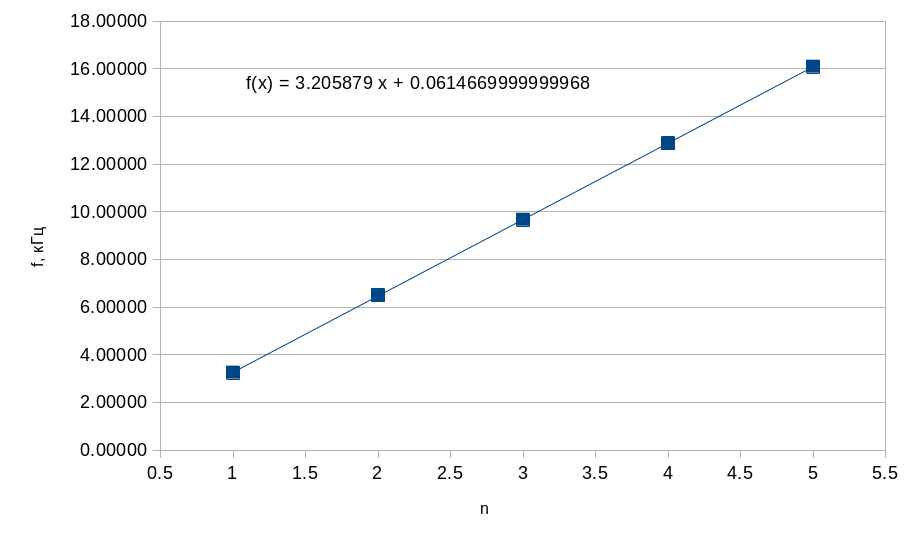
\includegraphics[scale=0.5]{med.png}
        \caption{Резонансы медного стержня}
    \end{figure}
    \begin{figure}[H]
        \centering
        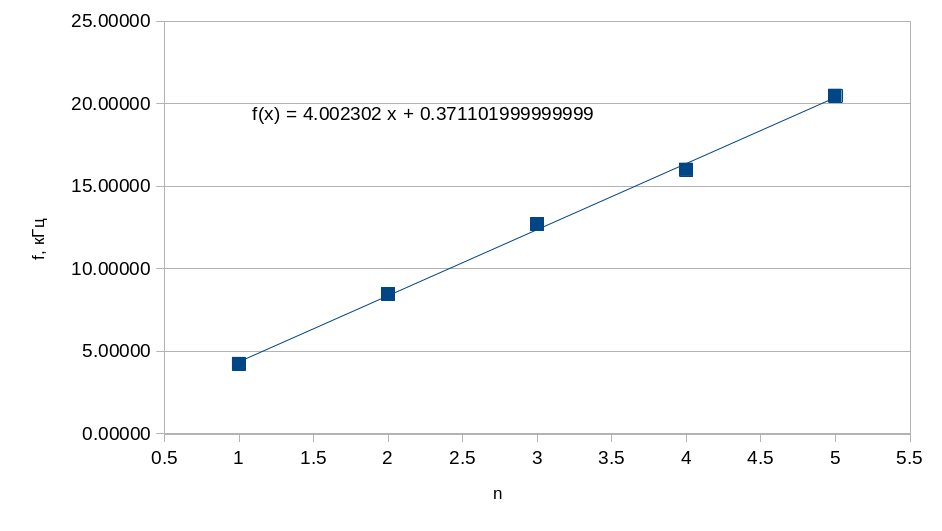
\includegraphics[scale=0.5]{dur.png}
        \caption{Резонансы дюралюминиевого стержня}
    \end{figure}
    \begin{figure}[H]
        \centering
        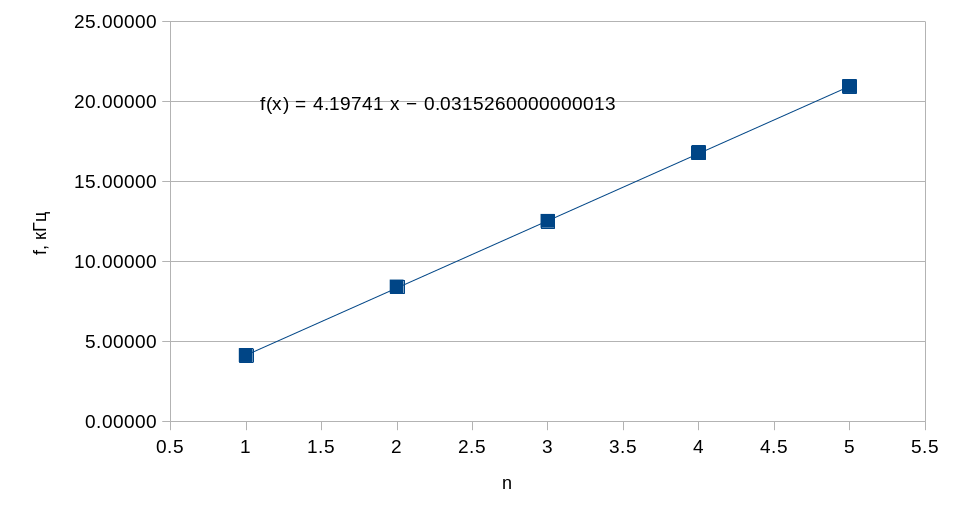
\includegraphics[scale=0.5]{steel.png}
        \caption{Резонансы стального стержня}
    \end{figure}

    \item По полученным угловым коэффициентам вычислим скорость распространения
    звуковой волны в стержнях, по которой найдем модуль Юнга.
    \begin{table}[H]
        \centering
        \caption{Рассчитанные угловые коэффициенты}
        \begin{tabular}{|c|c|c|c|}
        \hline
                     & Медь    & Дюралюминий & Сталь   \\ \hline
        $k$, кГц     & 3.20588 & 4.00230     & 4.19741 \\ \hline
        $v$, м/с     & 3847    & 4803        & 5037    \\ \hline
        $E$, Гпа     & 128     & 63          & 196     \\ \hline
        $\epsilon_k$ & 0.0010  & 0.0008      & 0.0005  \\ \hline
        $\epsilon_v$ & 0.0011  & 0.0009      & 0.0006  \\ \hline
        $\epsilon_E$ & 0.02    & 0.02        & 0.02    \\ \hline
        \end{tabular}
    \end{table}
    Таким образом, получаем итоговый результат:
    $$ E_{\text{меди}} = (128\pm3)\;\text{ГПа}, $$
    $$ E_{\text{дюр}}  = (63\pm2)\;\text{ГПа}, $$
    $$ E_{\text{ст}}   = (196\pm4)\;\text{ГПа} $$
    \item Проведем дополнительные измерения в окрестности 1-го резонанса
    для меди, чтобы получить добротность:
    $$ f_1 = (3.25178\pm0.00003)\; \text{кГц}, \\\ f_2 = (3.26688\pm0.00003)\; \text{кГц}, $$
    $$ \Delta f = 10.01\pm0.06\; \text{Гц}, $$
    $$ Q = \frac{f}{\Delta f} = 325 \pm 3$$
\end{enumerate}

    \section{Обсуждение результатов}
    В результате работы мы:
    \begin{enumerate}
        \item Нашли добротность медного стержня как колебательной системы.
        \item Получили зависимость $f(n)$. Как нетрудно убедиться по рис. 2 -- 4,
        во всех случаях аппроксимация прямой действительно применима, причем с очень
        хорошей точностью.
        \item Так как наше теоретическое предположение выполнилось, на его основе
        вычислили скорость звуковой волны во всех данных материалах.
        \item Нашли модули Юнга для меди, дюралюминия и стали.
        \item Если сравнить результаты с работой 1.3.1, где
        проводилось измерения методом прогиба, окажется, что точность опыта в данной
        работе существенно выше (в 1.3.1 мы получали погрешность порядка 10\%, тут
        около 2\%, причем наиболее существенный вклад в погрешность внесло измерение
        плотности). Такое расхождение можно объяснить высокой точностью измерения
        частоты по сравнению с точностью измерения деформаций в 1.3.1.
    \end{enumerate}

    \section{Вывод}
    Таким образом, их всего вышесказанного можно заключить, что использованный
    метод акустического резонанса куда лучше подходит для определения модуля
    Юнга, нежели метод прямых макродеформаций, использованный в работе 1.3.1.
    Точность получилось существенно выше. Кроме того, достаточно сделать точнее
    измерение плотности, чтобы снизить погрешность еще на несколько порядков.
\end{document}
